%%%%%%%%%%%%%%%%%%%%%%%%%%%%%%%%%%%%%%%%%%%%%%%%%%%%%%%%%%%%%%%%%%%%%%
%%                     Consumption
%%%%%%%%%%%%%%%%%%%%%%%%%%%%%%%%%%%%%%%%%%%%%%%%%%%%%%%%%%%%%%%%%%%%%%
%\color{blue}
\subsection{Glyph: \glyph{Consumption} }\label{sec:consumption}

\glyph{Consumption} is the arc used to represent the fact that an entity only affects a process,
but is not affected by it. 

\begin{glyphDescription}
 \item[SBO]\mbox{}\\ To be determined.
 \item[origin]\mbox{}\\ Any EPN (section \ref{sec:EPNs}).
 \item[target]\mbox{}\\ Any process node (section~\ref{sec:PNs}).
 \item[end-points]\mbox{}\\ No particular symbol is used to represent a source.
 \end{glyphDescription}


A cardinality label may be associated with \glyph{consumption} (section \ref{sec:consumption}) or 
\glyph{production} (section \ref{sec:production}) arc indicating the stoichiometry of a process. This label is a number enclosed in a rectangle with one of the long sides adjacent to the consumption arc. The cardinality is 
required to eliminate ambiguity when the exact composition, or the number of 
copies, of the inputs or outputs to a reaction are ambiguous from the diagram. 
An example is a multimer of 6 subunits dissociating into 2 monomers and 2 
dimers. Without stoichiometry labels another result, such as 4 monomers and 1 
dimer could be inferred. 
Once assigned to one arc of transition node, cardinality should be represented on
all \glyph{consumption} and \glyph{production} arcs connected to that transition
node to avoid misinterpretation.

Omitted cardinality on one edge only should not be treated as cardinality of 1, but
as unspecified cardinality. In most cases exact value could be derived from the
context, but unless cardinality is explicitly shown, it should be considered as
unspecified. In the case that stoichiometry of some part of the process is not
known, or undefined, question mark (?) should be used within cardinality label
of corresponding arcs.

\begin{figure}[H]
  \centering
  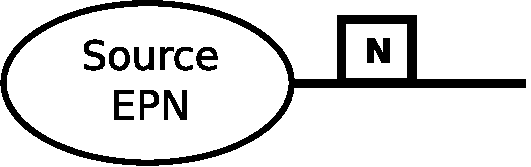
\includegraphics[scale = 0.5]{images/consumption}
  \caption{The \PD glyph for \glyph{consumption}.}
  \label{fig:consumption}
\end{figure}

